\documentclass{article}
\usepackage{amsmath, sfmath, multicol, tkz-euclide, array, enumerate, tcolorbox, tabularray}
\renewcommand{\familydefault}{\sfdefault}
\setlength{\parindent}{0cm}
\pagestyle{empty}
\usepackage[left=1in, top=0.5in, right=1in, bottom=0.5in]{geometry}
\tikzset{>=stealth}
\tcbset{colback=white}

\newcounter{example}[section]
\newenvironment{example}[1][]{\refstepcounter{example}\par\medskip
   {\color{red}\textbf{Example~\theexample. #1}}}{\medskip}

\begin{document}

\section*{Equations of Lines in the Coordinate Plane}

\begin{tcolorbox}[colframe=orange!70!white, coltitle=black, title=\textbf{Today I Can}]
\begin{enumerate}
    \item Graph and write linear equations.
\end{enumerate}
\end{tcolorbox}

\begin{tcolorbox}[colframe=black!20!white, opacitybacktitle=0.1, coltitle=black, title=\textbf{Slope}]

\begin{minipage}{0.5\textwidth}
\begin{itemize}
    \item $m = \frac{\text{rise}}{\text{run}} = \frac{y_2 - y_1}{x_2 - x_1}$
\end{itemize}
\end{minipage}
\begin{minipage}{0.4\textwidth}
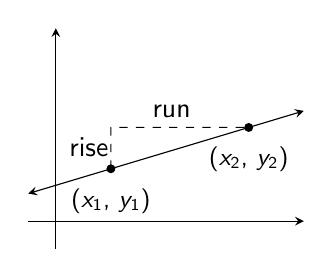
\begin{tikzpicture}[scale=0.7]
\draw [->, >=stealth] (0,0) -- (5,0);
\draw [->, >=stealth] (0.5,-0.5) -- (0.5,3.5);
\draw [<->, >=stealth] (0,0.5) -- (5,2);
\coordinate (A) at (1.5, 0.95);
\draw [fill=black] (A) circle (2pt);
\node at (A) [anchor = north, yshift=-0.05in] {\small $(x_1, \, y_1)$};
\coordinate (B) at (4, 1.7);
\draw [fill=black] (B) circle (2pt);
\node at (B) [anchor = north, yshift=-0.05in] {\small $(x_2, \, y_2)$};
\draw [dashed] (A) -- (1.5,1.7) -- (B);
\node at (1.1, 1.35) {rise};
\node at (2.6, 2) {run};
\end{tikzpicture}
\end{minipage}
\end{tcolorbox}

\begin{example}
What is the slope of the line that goes through the following pairs of points?
\begin{multicols}{2}
\begin{enumerate}[(a)]
    \item ($-1$, 2) and (4, $-2$)
    \item (4, 0) and (4, $-2$)
\end{enumerate}
\end{multicols}
\begin{minipage}{0.5\textwidth}
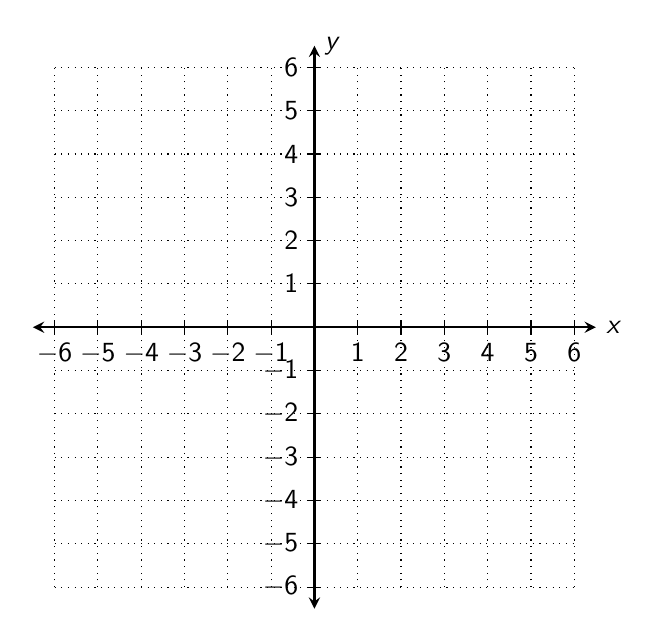
\begin{tikzpicture}[scale=0.55]
\draw[<->, thick] (-6.5,0) -- (6.5,0) node [right] {$x$};
\draw[<->, thick] (0,-6.5) -- (0,6.5) node [right] {$y$};
\draw[dotted] (-6,-6) grid (6,6);
\foreach \x in {-6,...,-1,,1,...,6}
\draw (\x, 0.15) -- (\x,-0.15) node [below] {$\tiny \x$};
\foreach \y in {-6,...,-1,,1,...,6}
\draw (0.15,\y) -- (-0.15,\y) node [left] {$\tiny \y$};
\end{tikzpicture}
\end{minipage}
\begin{minipage}{0.4\textwidth}
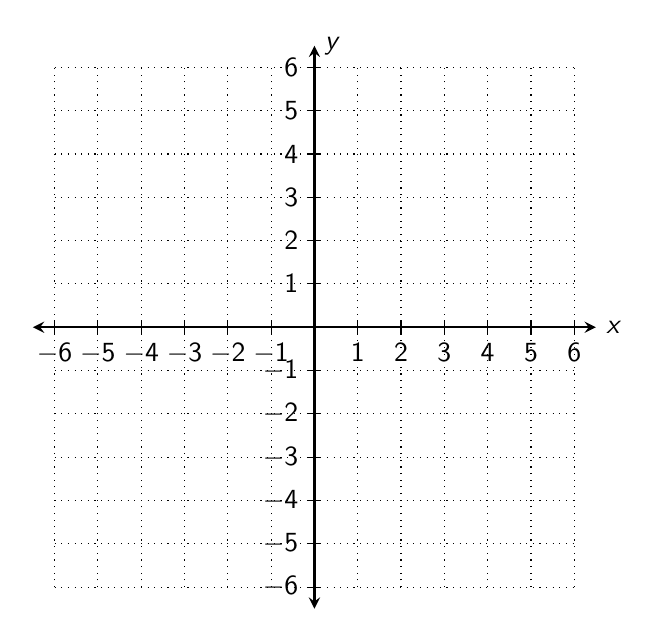
\begin{tikzpicture}[scale=0.55]
\draw[<->, thick] (-6.5,0) -- (6.5,0) node [right] {$x$};
\draw[<->, thick] (0,-6.5) -- (0,6.5) node [right] {$y$};
\draw[dotted] (-6,-6) grid (6,6);
\foreach \x in {-6,...,-1,,1,...,6}
\draw (\x, 0.15) -- (\x,-0.15) node [below] {$\tiny \x$};
\foreach \y in {-6,...,-1,,1,...,6}
\draw (0.15,\y) -- (-0.15,\y) node [left] {$\tiny \y$};
\end{tikzpicture}
\end{minipage}
\end{example}

\vfill 

\subsection*{Types of Slopes}

\begin{tabular}{p{0.2\textwidth}p{0.2\textwidth}p{0.2\textwidth}p{0.2\textwidth}}
Positive Slope  &   Negative Slope  &   Zero Slope  &   Undefined Slope  \\[0.2in]
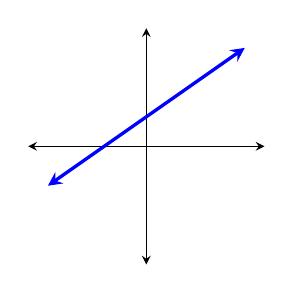
\begin{tikzpicture}
\draw [<->, >=stealth] (-1.5,0) -- (1.5,0);
\draw [<->, >=stealth] (0,-1.5) -- (0,1.5);
\draw [<->, >=stealth, very thick, blue] (-1.25,-0.5) -- (1.25,1.25);
\end{tikzpicture}
&
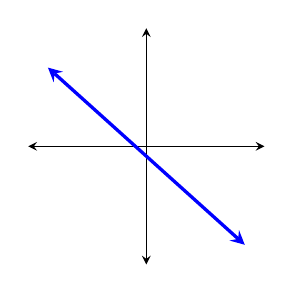
\begin{tikzpicture}
\draw [<->, >=stealth] (-1.5,0) -- (1.5,0);
\draw [<->, >=stealth] (0,-1.5) -- (0,1.5);
\draw [<->, >=stealth, very thick, blue] (-1.25,1) -- (1.25,-1.25);
\end{tikzpicture}
&
\begin{tikzpicture}
\draw [<->, >=stealth] (-1.5,0) -- (1.5,0);
\draw [<->, >=stealth] (0,-1.5) -- (0,1.5);
\draw [<->, >=stealth, very thick, blue] (-1.25,0.75) -- (1.25,0.75);
\end{tikzpicture}
&
\begin{tikzpicture}
\draw [<->, >=stealth] (-1.5,0) -- (1.5,0);
\draw [<->, >=stealth] (0,-1.5) -- (0,1.5);
\draw [<->, >=stealth, very thick, blue] (-0.5,-1.25) -- (-0.5,1.25);
\end{tikzpicture}
\end{tabular}

\vspace{0.25in}
\newpage 

\subsection*{Forms of Linear Equations}

\begin{tcolorbox}[colframe=black!20!white, opacitybacktitle=0.1, coltitle=black, title=\textbf{Slope-Intercept Form}]

\begin{itemize}
    \item $y = mx + b$
    \begin{itemize}
    \item Slope is $m$
    \item $y$-intercept is $b$
    \end{itemize}
\end{itemize}
\end{tcolorbox}

\begin{tcolorbox}[colframe=black!20!white, opacitybacktitle=0.1, coltitle=black, title=\textbf{Point-Slope Form}]

\begin{itemize}
    \item $y-y_1 = m(x-x_1)$
    \begin{itemize}
    \item Slope is $m$
    \item Point on the graph with coordinates $(x_1, y_1)$
    \end{itemize}
\end{itemize}
\end{tcolorbox}

\begin{example}
Graph each of the following.
\begin{multicols}{2}
\begin{enumerate}[(a)]
    \item $y = \frac{2}{3}x + 1$
    \item $y-2 = -\frac{1}{3}(x-1)$
\end{enumerate}    
\end{multicols}
\begin{minipage}{0.5\textwidth}
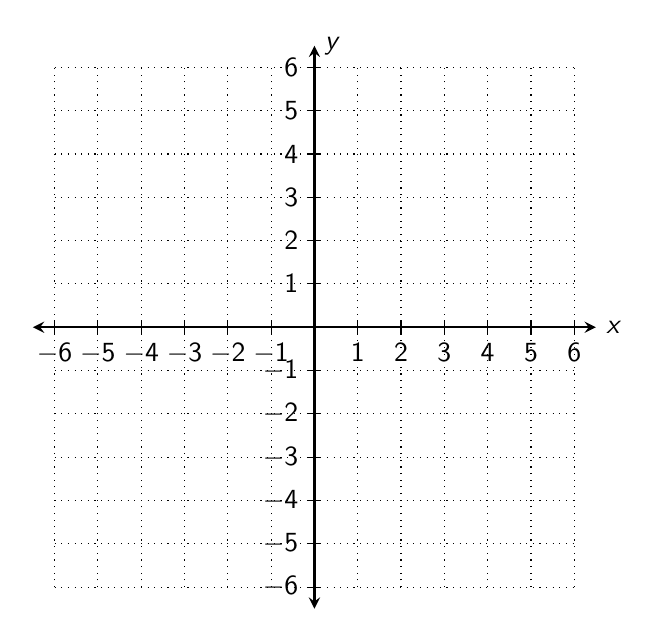
\begin{tikzpicture}[scale=0.55]
\draw[<->, thick] (-6.5,0) -- (6.5,0) node [right] {$x$};
\draw[<->, thick] (0,-6.5) -- (0,6.5) node [right] {$y$};
\draw[dotted] (-6,-6) grid (6,6);
\foreach \x in {-6,...,-1,,1,...,6}
\draw (\x, 0.15) -- (\x,-0.15) node [below] {$\tiny \x$};
\foreach \y in {-6,...,-1,,1,...,6}
\draw (0.15,\y) -- (-0.15,\y) node [left] {$\tiny \y$};
\end{tikzpicture}
\end{minipage}
\begin{minipage}{0.4\textwidth}
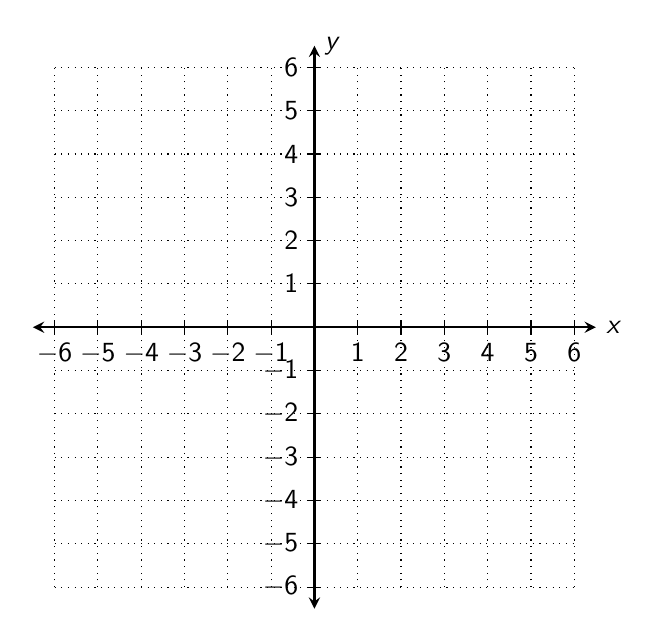
\begin{tikzpicture}[scale=0.55]
\draw[<->, thick] (-6.5,0) -- (6.5,0) node [right] {$x$};
\draw[<->, thick] (0,-6.5) -- (0,6.5) node [right] {$y$};
\draw[dotted] (-6,-6) grid (6,6);
\foreach \x in {-6,...,-1,,1,...,6}
\draw (\x, 0.15) -- (\x,-0.15) node [below] {$\tiny \x$};
\foreach \y in {-6,...,-1,,1,...,6}
\draw (0.15,\y) -- (-0.15,\y) node [left] {$\tiny \y$};
\end{tikzpicture}
\end{minipage}
\end{example}

\vspace{0.25in}

You can write the equation of a line when you know its slope and at least one point on the line.
\newline\\

\begin{example}
Write the equation of the line with each condition.
\begin{enumerate}[(a)]
    \item What is an equation of the line with slope 3 and $y$-intercept $-5$?  \vspace{0.75in} 
    \item What is an equation of the line through $(-1, \, 5)$ with slope 2?    \vfill 
\end{enumerate}
\end{example}

\newpage 

\begin{example}
Write the equation of the line that goes through each pair of points.
\begin{multicols}{2}
\begin{enumerate}[(a)]
    \item $(-2, \, -1)$ and (3, 5)
    \item (0, 3) and (2, 1)
\end{enumerate}
\end{multicols}
\begin{minipage}{0.5\textwidth}
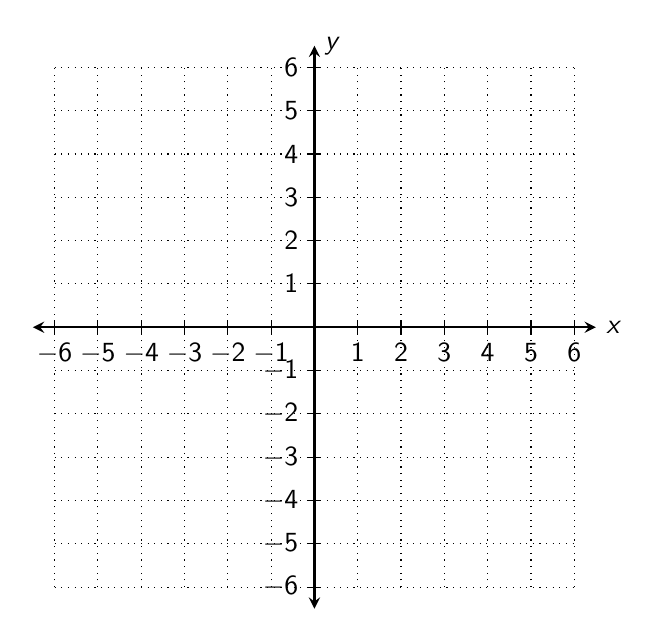
\begin{tikzpicture}[scale=0.55]
\draw[<->, thick] (-6.5,0) -- (6.5,0) node [right] {$x$};
\draw[<->, thick] (0,-6.5) -- (0,6.5) node [right] {$y$};
\draw[dotted] (-6,-6) grid (6,6);
\foreach \x in {-6,...,-1,,1,...,6}
\draw (\x, 0.15) -- (\x,-0.15) node [below] {$\tiny \x$};
\foreach \y in {-6,...,-1,,1,...,6}
\draw (0.15,\y) -- (-0.15,\y) node [left] {$\tiny \y$};
\end{tikzpicture}
\end{minipage}
\begin{minipage}{0.4\textwidth}
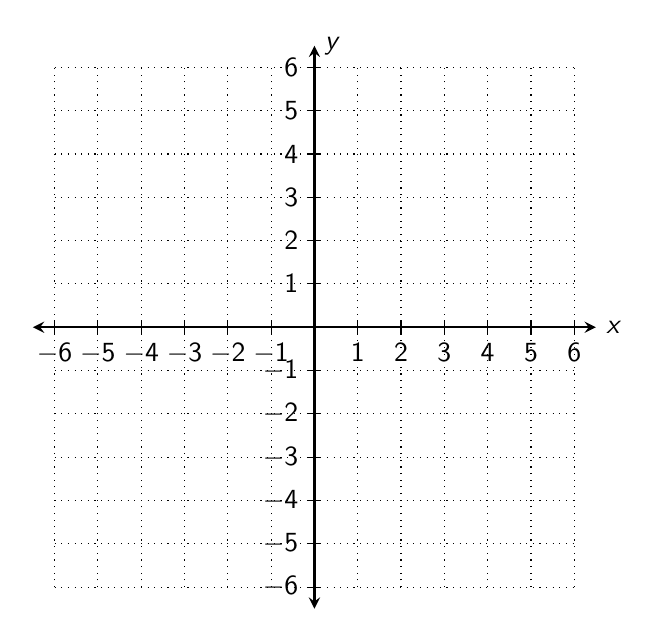
\begin{tikzpicture}[scale=0.55]
\draw[<->, thick] (-6.5,0) -- (6.5,0) node [right] {$x$};
\draw[<->, thick] (0,-6.5) -- (0,6.5) node [right] {$y$};
\draw[dotted] (-6,-6) grid (6,6);
\foreach \x in {-6,...,-1,,1,...,6}
\draw (\x, 0.15) -- (\x,-0.15) node [below] {$\tiny \x$};
\foreach \y in {-6,...,-1,,1,...,6}
\draw (0.15,\y) -- (-0.15,\y) node [left] {$\tiny \y$};
\end{tikzpicture}
\end{minipage}
\end{example}

\vfill 

\begin{example}
What are the equations of the horizontal and vertical lines through (2, 4)? \newline\\

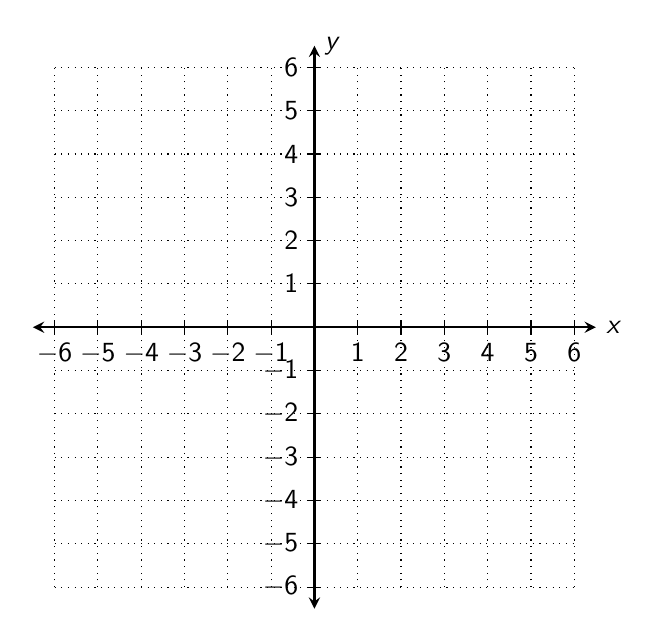
\begin{tikzpicture}[scale=0.55]
\draw[<->, thick] (-6.5,0) -- (6.5,0) node [right] {$x$};
\draw[<->, thick] (0,-6.5) -- (0,6.5) node [right] {$y$};
\draw[dotted] (-6,-6) grid (6,6);
\foreach \x in {-6,...,-1,,1,...,6}
\draw (\x, 0.15) -- (\x,-0.15) node [below] {$\tiny \x$};
\foreach \y in {-6,...,-1,,1,...,6}
\draw (0.15,\y) -- (-0.15,\y) node [left] {$\tiny \y$};
\end{tikzpicture}
\end{example}

\vfill 

\end{document}
